\documentclass{article}

\usepackage{fancyhdr}
\usepackage{extramarks}
\usepackage{amsmath}
\usepackage{amsthm}
\usepackage{amsfonts}
\usepackage{tikz}
\usepackage[plain]{algorithm}
\usepackage{algpseudocode}
\usepackage{enumerate}
\usepackage{graphicx}
\usepackage{pythonhighlight}
\usepackage{amssymb}
\usepackage{graphicx}
\usepackage{subfigure}

\usetikzlibrary{automata,positioning}

%
% Basic Document Settings
%  

\topmargin=-0.45in
\evensidemargin=0in
\oddsidemargin=0in
\textwidth=6.5in
\textheight=9.0in
\headsep=0.25in

\linespread{1.1}

\pagestyle{fancy}
\lhead{\hmwkAuthorName}
\chead{\hmwkClass\ (\hmwkClassInstructor): \hmwkTitle}
\rhead{\firstxmark}
\lfoot{\lastxmark}
\cfoot{\thepage}

\renewcommand\headrulewidth{0.4pt}
\renewcommand\footrulewidth{0.4pt}

\setlength\parindent{0pt}

%
% Create Problem Sections
%

\newcommand{\enterProblemHeader}[1]{
    \nobreak\extramarks{}{Problem \arabic{#1} continued on next page\ldots}\nobreak{}
    \nobreak\extramarks{Problem \arabic{#1} (continued)}{Problem \arabic{#1} continued on next page\ldots}\nobreak{}
}

\newcommand{\exitProblemHeader}[1]{
    \nobreak\extramarks{Problem \arabic{#1} (continued)}{Problem \arabic{#1} continued on next page\ldots}\nobreak{}
    \stepcounter{#1}
    \nobreak\extramarks{Problem \arabic{#1}}{}\nobreak{}
}

\setcounter{secnumdepth}{0}
\newcounter{partCounter}
\newcounter{homeworkProblemCounter}
\setcounter{homeworkProblemCounter}{1}
\nobreak\extramarks{Problem \arabic{homeworkProblemCounter}}{}\nobreak{}

%
% Homework Problem Environment
%
% This environment takes an optional argument. When given, it will adjust the
% problem counter. This is useful for when the problems given for your
% assignment aren't sequential. See the last 3 problems of this template for an
% example.
%
\newenvironment{homeworkProblem}[1][-1]{
    \ifnum#1>0
        \setcounter{homeworkProblemCounter}{#1}
    \fi
    \section{Problem \arabic{homeworkProblemCounter}}
    \setcounter{partCounter}{1}
    \enterProblemHeader{homeworkProblemCounter}
}{
    \exitProblemHeader{homeworkProblemCounter}
}

%
% Homework Details
%   - Title
%   - Due date
%   - Class
%   - Section/Time
%   - Instructor
%   - Author
%

\newcommand{\hmwkTitle}{Homework\ \#4}
\newcommand{\hmwkDueDate}{April 30, 2020}
\newcommand{\hmwkClass}{Reinforcement Learning}
\newcommand{\hmwkClassInstructor}{Professor Ziyu Shao}
\newcommand{\hmwkAuthorName}{Tianyuan Wu}
\newcommand{\hmwkAuthorID}{63305667}

%
% Title Page
%

\title{
    \vspace{2in}
    \textmd{\textbf{\hmwkClass:\ \hmwkTitle}}\\
    \normalsize\vspace{0.1in}\small{Due\ on\ \hmwkDueDate\ at 11:59am}\\
    \vspace{0.1in}\large{\textit{\hmwkClassInstructor}}
    \vspace{3in}
}

\author{\textbf{\hmwkAuthorName}\\ \hmwkAuthorID}
\date{}

\renewcommand{\part}[1]{\textbf{\large Part \Alph{partCounter}}\stepcounter{partCounter}\\}

%
% Various Helper Commands
%

% Useful for algorithms
\newcommand{\alg}[1]{\textsc{\bfseries \footnotesize #1}}

% For derivatives
\newcommand{\deriv}[1]{\frac{\mathrm{d}}{\mathrm{d}x} (#1)}

% For partial derivatives
\newcommand{\pderiv}[2]{\frac{\partial}{\partial #1} (#2)}

% Integral dx
\newcommand{\dx}{\mathrm{d}x}

% Alias for the Solution section header
\newcommand{\solution}{\textbf{\large Solution}}

% Probability commands: Expectation, Variance, Covariance, Bias
\newcommand{\E}{\mathrm{E}}
\newcommand{\Var}{\mathrm{Var}}
\newcommand{\Cov}{\mathrm{Cov}}
\newcommand{\Bias}{\mathrm{Bias}}

\begin{document}

\maketitle

\pagebreak

\begin{homeworkProblem}
    \textbf{Solution}\\
    To get the average number of 1s in good sequences, we can apply MCMC method.\\
    \begin{enumerate}
        \item Init the sequence to $(000\ldots 0)_n$.
        \item Generate a random number $k = [0, n-1]$, and filp the bit at index $k$.
        \item If the new sequence is a good sequence, goto the new sequence; Otherwise stay at the same position.
        \item Jump to step (2).
    \end{enumerate}
    The length of the sequence is set to 100, then we can obtain the expected number of 1s in good sequence is $27.727864$, 
    which is very close to the real value.
\end{homeworkProblem}


\begin{homeworkProblem}
    \textbf{Solution}\\
    We can generate the power-law distribution (using MH method) by following steps:
    \begin{enumerate}
        \item Construct a Markov chain with 
        $$P = \{p_{ij}\} = \begin{cases}1,\quad i==1\ and\ j==1\\ \frac{1}{2},\quad otherwise\end{cases}$$
        \item Start at a random state (or a given state), called $s_0$.
        \item Determine a proposal state $s'$ according to $P$.
        \item Filp a coin with probability of landing head $p_H = \min\{1, \frac{p_{ij}\pi_i}{p_{ji}\pi_j}\}$
        \item If the coin landing head, accept the proposal, otherwise reject the proposal.
        \item Jump to step (2)
    \end{enumerate}
    The simulation results are shown below, \textbf{the right-most bar of the histogram (i.e. The bar with subscript 9) means $i \ge 9$} 
    \begin{table}[H]
        \begin{center}
        \begin{tabular}{c|c}
            X & P\\
            \hline\hline
            1 & 0.390231\\
            2 &  0.137773\\
            3 &  0.075105\\
            4 &  0.048989\\
            5 &  0.035108\\
            6 &  0.026976\\
            7 &  0.021640\\
            8 &  0.017884\\
            $\ge$ 9 &  0.246295\\
        \end{tabular}
        \end{center}
    \end{table}

    \begin{figure}[h]
        \begin{center}
        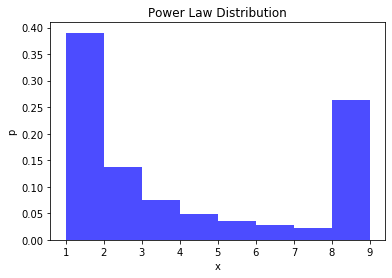
\includegraphics[scale=0.5]{powerlaw.png}
        \end{center}
    \end{figure}
\end{homeworkProblem}

\begin{homeworkProblem}
    \textbf{Solution}\\
    We can solve Knapsack's problem (using MH method) by following steps:
    \begin{enumerate}
        \item Init the sequence to $s_i =(000\ldots 0)_n$.
        \item Generate a random number $k = [0, n-1]$, and filp the bit at index $k$, to get the new state $s_{new}$.
        \item If the new sequence satisfies $\sum_i{s_iw_i} > w$, stay at current position.
        \item Let $V_{s_i} = \sum_i{s_i g_i}$, filp a coin with probability of landing head $p = e^{\beta(V_{new} - V_{curr})}$
        \item If the coin landing head, accept the proposal, otherwise reject the proposal.
        \item Jump to step (2)
    \end{enumerate}
    The simulation result for $m=5$, $w=10$, vector of worth $\{g_j\}=(6,3,5,4,6)$, vector of weight $\{w_j\}=(2,2,6,5,4)$
    is: the best solution is $11001$ (i.e. choose the item with index 1,2,5), and the maximum worth is 15.0.
\end{homeworkProblem}


\begin{homeworkProblem}
    \textbf{Solution}\\
    We can generate the standard normal distribution (using MH method) by following steps:
    \begin{enumerate}
        \item Generate a random number by $w = Unif(0, 1)$ as state $w_0$
        \item Generate a new random number by $u = Unif(0, 1)$.
        \item Filp a coin with probability of landing head $p_H = \min\{1, \frac{e^{-\frac{1}{2}u^2}}{e^{-\frac{1}{2}w^2}}\}$
        \item If the coin landing head, accept the proposal (set $w=u$), otherwise reject the proposal (stay at $w$).
        \item Jump to step (2)
    \end{enumerate}
    \textbf{Comparison}:\\
    - The Box-Muller method can generate 2 independent normal distributions at the same time, but if we only want 1 
      normal distribution, we also need 2 uniform distribution samples for one normal distribution sample ($\sqrt{-log(u_1)}cos(2\pi u_2)$).\\
    - But by using MH method, we can only using 1 uniform distribution sample to generate a normal distribution sample.\\
    The simulation results are shown below:
    \begin{figure}[h]
        \begin{center}
        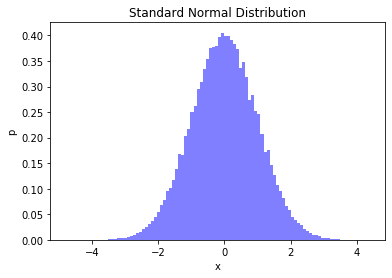
\includegraphics[scale=0.5]{normal.png}
        \end{center}
    \end{figure}
\end{homeworkProblem}


\begin{homeworkProblem}
    \textbf{Solution}\\
    We can generate the beta distribution (using MH method) by following steps:
    \begin{enumerate}
        \item Generate a random number by $w = Unif(0, 1)$ as state $w_0$
        \item Generate a new random number by $u = Unif(0, 1)$.
        \item Filp a coin with probability of landing head $p_H = \min\{1, \frac{u^{a-1}(1-u)^{b-1}}{w^{a-1}(1-w)^{b-1}}\}$
        \item If the coin landing head, accept the proposal (set $w=u$), otherwise reject the proposal (stay at $w$).
        \item Jump to step (2)
    \end{enumerate}
    The simulation result (with parameters $a=5, b=5$) are shown below:
    \begin{figure}[h]
        \begin{center}
        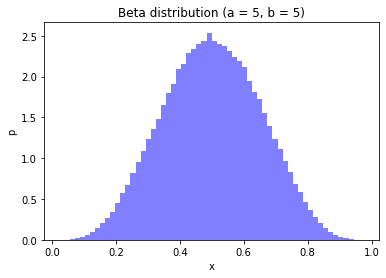
\includegraphics[scale=0.5]{beta.png}
        \end{center}
    \end{figure}
\end{homeworkProblem}


\begin{homeworkProblem}
    \textbf{Solution}\\
    We can solve the Normal-Normal conjugacy problem (using MH method) by following steps:
    \begin{enumerate}
        \item Generate a random number by $w = Norm(\mu, \sigma^2)$ as state $w_0$
        \item Generate a new random number by $u = w + \mathcal{N}(0, d^2)$.
        \item Filp a coin with probability of landing head 
        $$p_H = \min\{1, \frac{e^{-\frac{1}{2\sigma^2}(y-u)^2} e^{-\frac{1}{2\tau^2}(u-\mu)^2}}{e^{-\frac{1}{2\sigma^2}(y-w)^2} e^{-\frac{1}{2\tau^2}(w-\mu)^2}}\}$$
        \item If the coin landing head, accept the proposal (set $w=u$), otherwise reject the proposal (stay at $w$).
        \item Jump to step (2)
    \end{enumerate}
    The simulation results are shown below:
    \begin{figure}[htbp]
        \centering

        \subfigure[d=0.1]{
        \begin{minipage}[t]{0.3\linewidth}
        \centering
        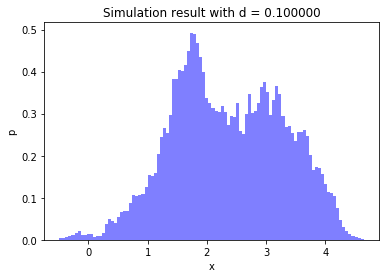
\includegraphics[width=1.8in]{norm01.png}
        %\caption{fig1}
        \end{minipage}%
        }%
        \subfigure[d=0.5]{
        \begin{minipage}[t]{0.3\linewidth}
        \centering
        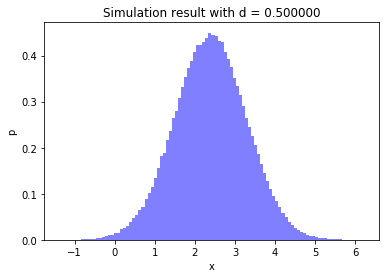
\includegraphics[width=1.8in]{norm05.png}
        %\caption{fig2}
        \end{minipage}%
        }%
        \subfigure[d=1]{
        \begin{minipage}[t]{0.3\linewidth}
        \centering
        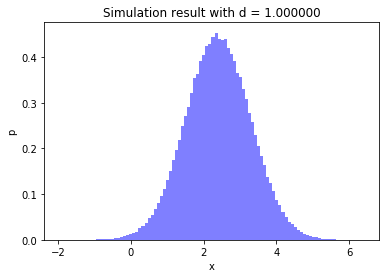
\includegraphics[width=1.8in]{norm1.png}
        %\caption{fig2}
        \end{minipage}%
        }%
                        
        \subfigure[d=5]{
        \begin{minipage}[t]{0.3\linewidth}
        \centering
        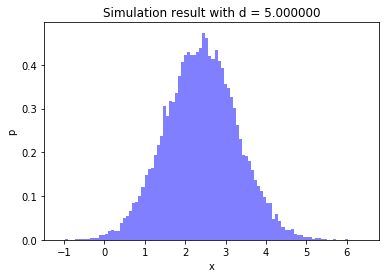
\includegraphics[width=1.8in]{norm5.png}
        %\caption{fig2}
        \end{minipage}%
        }%
        \subfigure[d=10]{
        \begin{minipage}[t]{0.3\linewidth}
        \centering
        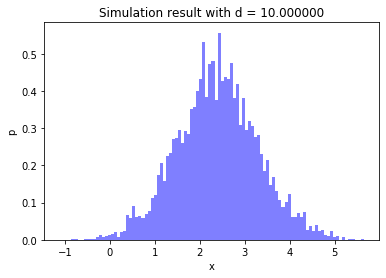
\includegraphics[width=1.8in]{norm10.png}
        %\caption{fig2}
        \end{minipage}%
        }%
        \subfigure[d=100]{
        \begin{minipage}[t]{0.3\linewidth}
        \centering
        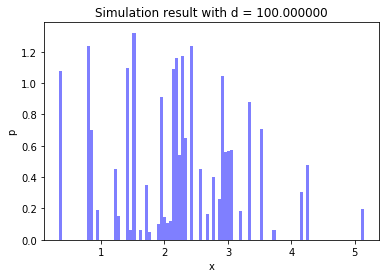
\includegraphics[width=1.8in]{norm100.png}
        %\caption{fig2}
        \end{minipage}%
        }%
        
        \centering
        \caption{Simulation results}
    \end{figure}
\end{homeworkProblem}


\begin{homeworkProblem}
    \textbf{Solution}\\
    We can generate the bivariate normal distribution (using Gibbs method) by following steps:
    \begin{enumerate}
        \item Init $x=0$, $y=0$
        \item Update $x=\mathcal{N}(\rho y, 1-\rho^2)$
        \item Update $y=\mathcal{N}(\rho x, 1-\rho^2)$
        \item Jump to step (2)
    \end{enumerate}
    The simulation result (with parameters $\rho=0.6$ and $\rho=-0.6$) are shown below:
    \begin{figure}[H]
        \begin{center}
        \caption{$\rho=0.6$}
        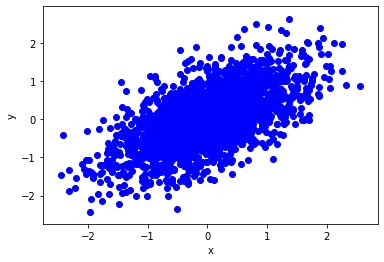
\includegraphics[scale=0.5]{biv1.png}
        \end{center}
    \end{figure}
    \begin{figure}[H]
        \begin{center}
        \caption{$\rho=-0.6$}
        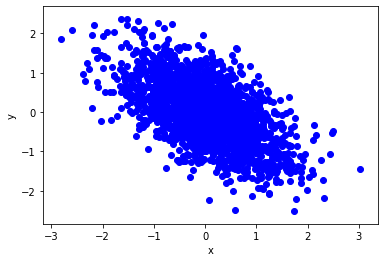
\includegraphics[scale=0.5]{biv2.png}
        \end{center}
    \end{figure}
\end{homeworkProblem}


\begin{homeworkProblem}
    \textbf{Solution}\\
    We can solve the Normal-Normal conjugacy problem (using MH method or Gibbs sampling) by following steps:\\
    \textbf{MH}:
    \begin{enumerate}
        \item Generate a random number by $w \sim Beta(a,b)$ as state $w_0$
        \item Generate a new random number by $u \sim Beta(a,b)$
        \item Filp a coin with probability of landing head 
        $$p_H = \min\{1, \frac{e^{\lambda u}(\lambda u)^x u^{a-1}(1-u)^{b-1}}{e^{\lambda w}(\lambda w)^x w^{a-1}(1-w)^{b-1}}   \}$$
        \item If the coin landing head, accept the proposal (set $w=u$), otherwise reject the proposal (stay at $w$).
        \item Jump to step (2)
    \end{enumerate}
    \textbf{Gibbs}:
    \begin{enumerate}
        \item Init $n$ to some random value or given value
        \item Generate a $p \sim Beta(x+a, n-x+b)$
        \item Sample $y \sim Pois(\lambda(1-p))$
        \item Update $n = x + y$
        \item Jump to step (2)
    \end{enumerate}

    \textbf{Comparsion}:\\
    - The MH method is actually a accept-reject method, if the simulation steps are not enough, it may reject many times 
      and stay at the same state, also, it may need more calculations.\\
    - The Gibbs sampling need less calculations, but the choice of systemic or random scan may effects the simulation results.\\

    The simulation results are shown below:\\
    \textbf{MH method}:\\
    \begin{figure}[h]
        \begin{center}
        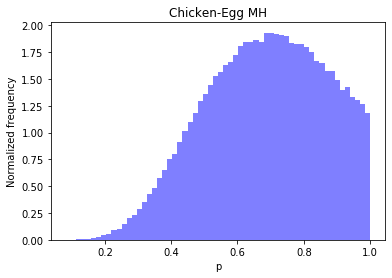
\includegraphics[scale=0.5]{cemh.png}
        \end{center}
    \end{figure}
    The parameters of $p$: Mean: 0.6848, Variance: 0.0320 \\
    \textbf{Gibbs method}:\\
    \begin{figure}[h]
        \begin{center}
        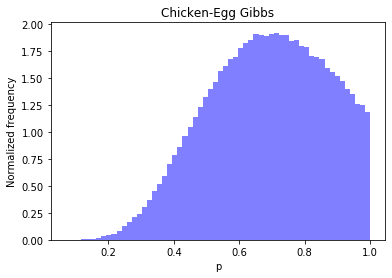
\includegraphics[scale=0.5]{cegb.png}
        \end{center}
    \end{figure}
    The parameters of $p$: Mean: 0.6850, Variance: 0.0319 \\
\end{homeworkProblem}


\begin{homeworkProblem}
    \textbf{Solution}\\
    We can generate the three dimensional joint distribution (using Gibbs sampling) by following steps:\\
    \textbf{MH}:
    \begin{enumerate}
        \item Init $(x_0, p_0, n_0) \gets (1,0.5,2) $
        \item Generate $x_m \sim Bino(n_{m-1}, p_{m-1})$
        \item Generate $p_m \sim Beta(x_m +1,  n_{m-1}-x_m +1)$
        \item Generate $n_m = x_m + z$, where $z \sim Pois(4(1-p_m))$
        \item Jump to step (2)
    \end{enumerate}
    \begin{figure}[htbp]
        \centering

        \subfigure[x-n]{
        \begin{minipage}[t]{0.5\linewidth}
        \centering
        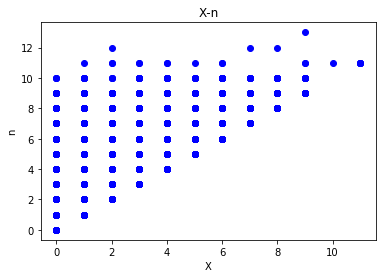
\includegraphics[width=2.5in]{xn.png}
        %\caption{fig1}
        \end{minipage}%
        }%
        \subfigure[x-p]{
        \begin{minipage}[t]{0.5\linewidth}
        \centering
        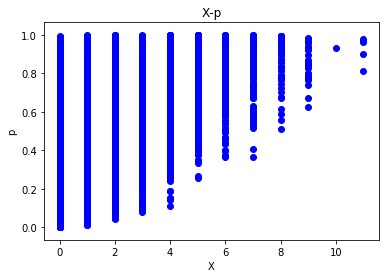
\includegraphics[width=2.5in]{xp.png}
        %\caption{fig2}
        \end{minipage}%
        }%
                        
        \subfigure[p-n]{
        \begin{minipage}[t]{0.5\linewidth}
        \centering
        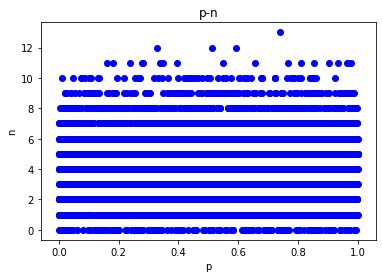
\includegraphics[width=2.5in]{pn.png}
        %\caption{fig2}
        \end{minipage}%
        }%
        \subfigure[x-p-n]{
        \begin{minipage}[t]{0.5\linewidth}
        \centering
        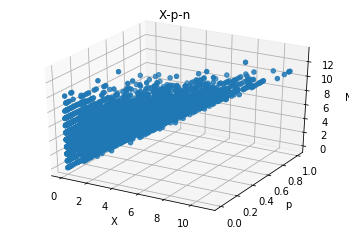
\includegraphics[width=2.5in]{xpn.png}
        %\caption{fig2}
        \end{minipage}%
        }%
        
        \centering
        \caption{Simulation results}
        \end{figure}
\end{homeworkProblem}

\begin{homeworkProblem}
    \textbf{Solution}\\
    \textbf{(a) Discrete Time}\\
    First, we analysis the problem theoretically. The independent set problem is quite similar like the Knapsack problem, and we can solve 
    it by similar ways. The basic idea is, use a binary sequence to represent the choice of independent set. $s[i] = 1$ means choose vertex 
    $i$, and $s[i] = 0$ means not choose. Then, construct a irreducible Markov Chain, each sate $X_i$ represent a binary sequence, and in each iteration, 
    we filp a bit randomly, if the new sequence does not satisfy the independent set constraint, stay at the current state, otherwise go to 
    the new state. Then, the stationary distribution $\pi$ of this chain is an uniform distribution. Then, we can modify the chain to make 
    it concentrate on states with larger size of independent set (i.e. larger number of 1s), by MH method. That is, filp a coin with 
    $p_H = e^{\beta(V_{new} - V_{curr})}$, where $V_{s_i} = \#\ of\ 1s\ in\ s_i$. Then if the coin landing head, accept the proposal, otherwise 
    reject the proposal.\\
    
    That idea can be described in details as:
    \begin{enumerate}
        \item Label all vertices by a number $0, 1, \ldots, n$
        \item Init the sequence to $s_i =(000\ldots 0)_n$, $0$ means the vertex is not in the independent set, and $1$ means it's in the set.
        \item Generate a random number $k = [0, n-1]$, and filp the bit at index $k$, to get the new state $s_{new}$.
        \item If the new sequence not satisfies the constraint of independent set (i.e. Exists 2 adjacent vertices are both ``1'' in new sequence), stay at current position.
        \item Let $V_{s_i} = \#\ of\ 1s\ in\ s_i$, filp a coin with probability of landing head $p = e^{\beta(V_{new} - V_{curr})}$
        \item If the coin landing head, accept the proposal, otherwise reject the proposal.
        \item Jump to step (3)
    \end{enumerate}
    We do simulation $5\times 10^5$ steps, and we can observe the maximum size of the independent set is $8$,
    we run it several times, and some of the simulation results are shown below:  \newline\newline
    \textbf{The choice of maximum independent set is: 000101001010010010010101, with size = 9\\
            The choice of maximum independent set is: 010000011010101010100100, with size = 9\\}
    \newline
    The result is the same as the optimal solution (size=9).
    \newline

    \textbf{(b) Continuous time}\\
    The basic idea is similar to the discrete time solution, the only difference is, the time is continuous. If the chain at 
    state $s_i$, and a proposal state $s_j$. Then the transfer time $t_{trans} \sim f(V_{s_i})$, where 
    $f$ is a distribution with parameter $V_{s_i}$. That is, we want the chain stay at high value states longer, and spend
    little time on states with lower value. Here we use $t_{trans} \sim Pois(V_{s_i})$\\
    That idea can be described in details as:
    \begin{enumerate}
        \item Consider $G(V,E)$ is the graph that we want to find the independent set. 
        \item Let $X_0$ is an arbitrary independent set of $G$ (we can choose a vertex as $X_0$ in practice).
        \item Then we compute $X_{i+1}$, first we choose a vertex $v$ uniformly at random from $V$
        \item If $v \in X_{i}$, then set $X_{i+1} = X_{i} \setminus v$ with probability $min(1, \frac{1}{\lambda})$, otherwise set $X_{i+1} = X_{i}$
        \item If $v \notin X_{i}$, and adding $v$ to $X_{i}$ still gives an independent set, then set $X_{i+1} = X_{i} \cup v$, with probability $min(1, \lambda)$, otherwise set $X_{i+1} = X_{i}$
        \item Jump to step (3)
    \end{enumerate}
    We do simulation $5\times 10^5$ steps, and we can observe the maximum size of the independent set is $8$,
    we run it several times, and some of the simulation results are shown below:  \newline\newline
    \textbf{The choice of maximum independent set is: 000101101000001010010101, with size = 9\\}
    \newline
    Which is the same as the DTMC result.
    \newline

    \textbf{(c) Comparison}
    \begin{itemize}
        \item DTMC:\\
            - Pros: This method make the chain stay at states with high values with higher probability. It's easy to 
              implement and can converge to the optimal value fast (if $\beta$ is set properly). \\
            - Cons: Due to the extremely large state space ($2^24$ in this problem), if the simulation steps are not 
              enough, it may be ``locked'' on some sub-optimal states .
        \item Continuous Time:\\
            - Pros: The time is continuous, and the time it stay on some state is determined by the value of the state. 
              It may have better performance than DTMC for it will not ``locked'' on some sub-optimal state.\\
            - Cons: Due to the time is continuous, it's hard to implement, and it may converge slower than DTMC.
    \end{itemize}
\end{homeworkProblem}

\end{document}
